Another important type of latent variable models are latent growth curve
models. Growth modeling is often used to analyze longitudinal or
developmental data. In this type of data, an outcome measure is measured
on several occasions, and we want to study the change over time. In many
cases, the trajectory over time can be modeled as a simple linear or
quadratic curve. Random effects are used to capture individual
differences. The random effects are conveniently represented by
(continuous) latent variables, often called \emph{growth factors}. In
the example below, we use an artifical dataset called
\texttt{Demo.growth} where a score (say, a standardized score on a
reading ability scale) is measured on 4 time points. To fit a linear
growth model for these four time points, we need to specify a model with
two latent variables: a random intercept, and a random slope:

\begin{verbatim}
# linear growth model with 4 timepoints
# intercept and slope with fixed coefficients
 i =~ 1*t1 + 1*t2 + 1*t3 + 1*t4
 s =~ 0*t1 + 1*t2 + 2*t3 + 3*t4
\end{verbatim}

In this model, we have fixed all the coefficients of the growth
functions. If \texttt{i} and \texttt{s} are the only `latent variables'
in the model, we can use the \texttt{growth()} function to fit this
model:

\begin{Shaded}
\begin{Highlighting}[]
\NormalTok{model }\OtherTok{\textless{}{-}} \StringTok{\textquotesingle{} i =\textasciitilde{} 1*t1 + 1*t2 + 1*t3 + 1*t4}
\StringTok{           s =\textasciitilde{} 0*t1 + 1*t2 + 2*t3 + 3*t4 \textquotesingle{}}
\NormalTok{fit }\OtherTok{\textless{}{-}} \FunctionTok{growth}\NormalTok{(model, }\AttributeTok{data=}\NormalTok{Demo.growth)}
\FunctionTok{summary}\NormalTok{(fit)}
\end{Highlighting}
\end{Shaded}

\begin{verbatim}
lavaan 0.6-11 ended normally after 29 iterations

  Estimator                                         ML
  Optimization method                           NLMINB
  Number of model parameters                         9
                                                      
  Number of observations                           400
                                                      
Model Test User Model:
                                                      
  Test statistic                                 8.069
  Degrees of freedom                                 5
  P-value (Chi-square)                           0.152

Parameter Estimates:

  Standard errors                             Standard
  Information                                 Expected
  Information saturated (h1) model          Structured

Latent Variables:
                   Estimate  Std.Err  z-value  P(>|z|)
  i =~                                                
    t1                1.000                           
    t2                1.000                           
    t3                1.000                           
    t4                1.000                           
  s =~                                                
    t1                0.000                           
    t2                1.000                           
    t3                2.000                           
    t4                3.000                           

Covariances:
                   Estimate  Std.Err  z-value  P(>|z|)
  i ~~                                                
    s                 0.618    0.071    8.686    0.000

Intercepts:
                   Estimate  Std.Err  z-value  P(>|z|)
   .t1                0.000                           
   .t2                0.000                           
   .t3                0.000                           
   .t4                0.000                           
    i                 0.615    0.077    8.007    0.000
    s                 1.006    0.042   24.076    0.000

Variances:
                   Estimate  Std.Err  z-value  P(>|z|)
   .t1                0.595    0.086    6.944    0.000
   .t2                0.676    0.061   11.061    0.000
   .t3                0.635    0.072    8.761    0.000
   .t4                0.508    0.124    4.090    0.000
    i                 1.932    0.173   11.194    0.000
    s                 0.587    0.052   11.336    0.000
\end{verbatim}

Technically, the \texttt{growth()} function is almost identical to the
\texttt{sem()} function. But a mean structure is automatically assumed,
and the observed intercepts are fixed to zero by default, while the
latent variable intercepts/means are freely estimated. A slightly more
complex model adds two regressors (\texttt{x1} and \texttt{x2}) that
influence the latent growth factors. In addition, a time-varying
covariate \texttt{c} that influences the outcome measure at the four
time points has been added to the model. A graphical representation of
this model is presented below.

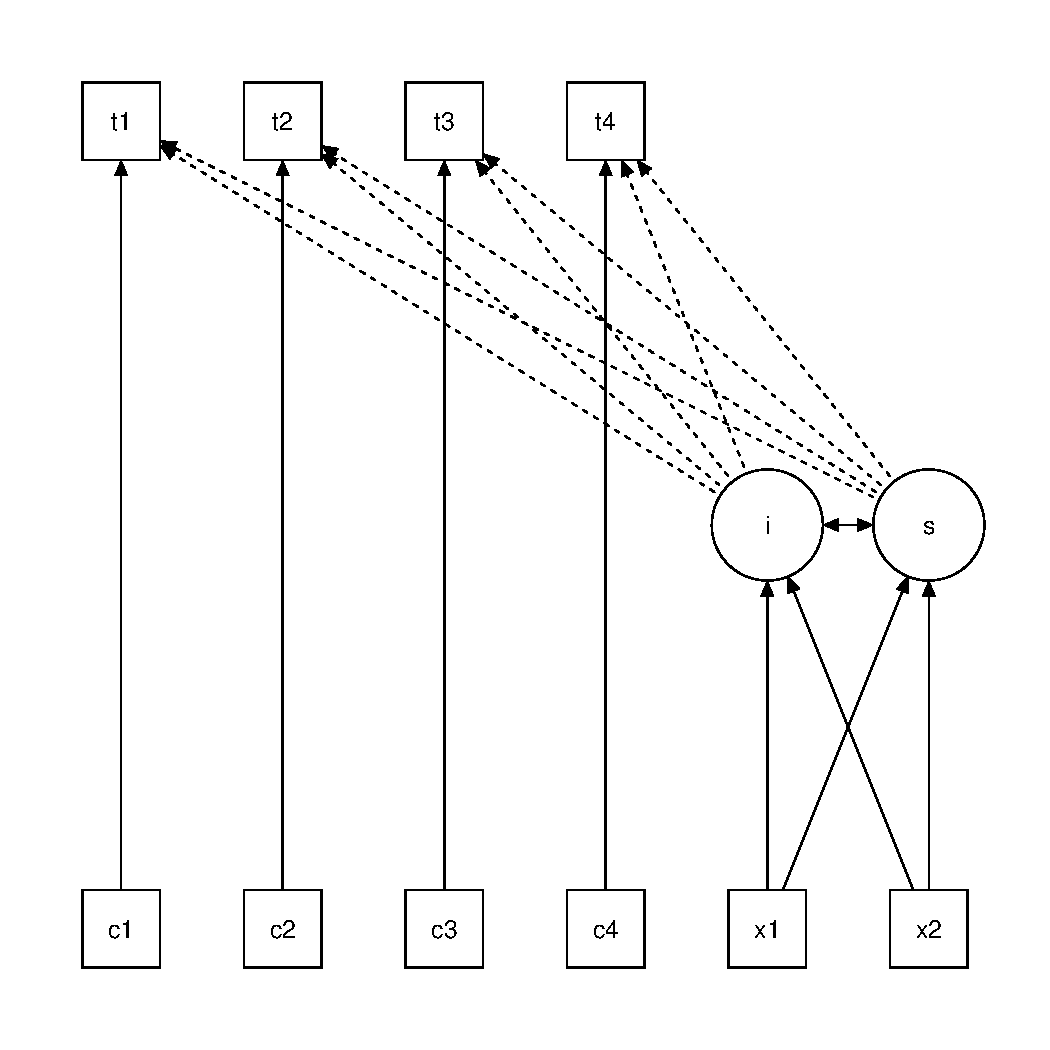
\includegraphics{figure/growth-1.pdf}

The complete R code needed to specify and fit this linear growth model
with a time-varying covariate is given below:

\begin{Shaded}
\begin{Highlighting}[]
\CommentTok{\# a linear growth model with a time{-}varying covariate}
\NormalTok{model }\OtherTok{\textless{}{-}} \StringTok{\textquotesingle{}}
\StringTok{  \# intercept and slope with fixed coefficients}
\StringTok{    i =\textasciitilde{} 1*t1 + 1*t2 + 1*t3 + 1*t4}
\StringTok{    s =\textasciitilde{} 0*t1 + 1*t2 + 2*t3 + 3*t4}
\StringTok{  \# regressions}
\StringTok{    i \textasciitilde{} x1 + x2}
\StringTok{    s \textasciitilde{} x1 + x2}
\StringTok{  \# time{-}varying covariates}
\StringTok{    t1 \textasciitilde{} c1}
\StringTok{    t2 \textasciitilde{} c2}
\StringTok{    t3 \textasciitilde{} c3}
\StringTok{    t4 \textasciitilde{} c4}
\StringTok{\textquotesingle{}}
\NormalTok{fit }\OtherTok{\textless{}{-}} \FunctionTok{growth}\NormalTok{(model, }\AttributeTok{data =}\NormalTok{ Demo.growth)}
\FunctionTok{summary}\NormalTok{(fit)}
\end{Highlighting}
\end{Shaded}
